\documentclass[12pt, twosided]{article}

\usepackage[letterpaper,bindingoffset=0in,%
            left=1in,right=1in,top=1in,bottom=1in,%
            footskip=.25in]{geometry}

\usepackage{mathtools}
\usepackage{graphicx}

\usepackage{setspace}
\setstretch{1.1}

\usepackage{amsmath}
\usepackage{amsfonts}
\usepackage{amsthm}
\usepackage{amssymb}
\usepackage{csquotes}
\usepackage{relsize}

\usepackage{tikz}
\usetikzlibrary{cd}
\usetikzlibrary{fit,shapes.geometric}
\tikzset{%  
    mdot/.style={draw, circle, fill=black},
    mset/.style={draw, ellipse, very thick},
}

\usepackage{hhline}
\usepackage{systeme}
\usepackage{mathrsfs}
\usepackage{hyperref}
\usepackage{mathtools}  
\usepackage{silence}
\usepackage{blkarray}
\usepackage{float}
\usepackage{framed}
\usepackage{array}
\usepackage{stmaryrd}
\usepackage{extarrows}
\usepackage{caption}
\captionsetup[figure]{labelfont={bf},name={Fig.},labelsep=period}

\theoremstyle{definition}
\newtheorem{df}{Definition}
\newtheorem{exa}{Example}
\newtheorem{ques}{Question}
\newtheorem{exr}{Exercise}
\newtheorem*{note}{Note}
\theoremstyle{plain}
\newtheorem{thm}{Theorem}
\newtheorem{prop}{Proposition}
\newtheorem{conj}{Conjecture}
\newtheorem{cor}{Corollary}
\newtheorem{lm}{Lemma}
\newtheorem*{fact}{Fact}
\newtheorem*{idea}{Idea}
\newtheorem*{clm}{Claim}
\newtheorem*{rmk}{Remark}
\usepackage[ruled]{algorithm2e}

\usepackage{ulem}
\makeatletter

\def\lf{\left\lfloor}   
\def\rf{\right\rfloor}
\def\lc{\left\lceil}   
\def\rc{\right\rceil}
\def\st{\text{ s.t. }}
\def\1{^{-1}}
\def\ind{\mathbf{1}}
\def\R{\mathbb{R}}
\def\Q{\mathbb{Q}}
\def\Z{\mathbb{Z}}
\def\C{\mathbb{C}}
\def\I{\mathbb{I}}
\def\N{\mathbb{N}}
\def\F{\mathbb{F}}
\def\A{\mathbb{A}}
\def\Li{\text{Li}}
\def\th{^\text{th}}
\def\sp{\text{Sp}}
\def\opn{\left\{}
\def\cls{\right\}}
\def\Aut{\text{Aut}}
\def\PG{\text{PG}}
\def\GL{\text{GL}}
\def\PGL{\text{PGL}}
\def\Cov{\text{Cov}}
\def\Pack{\text{Pack}}
\def\PgamL{\text{P}\Gamma\text{L}}
\def\gamL{\Gamma\text{L}}
\def\cl{\text{cl}}
\def\stbar{\ \middle\vert\ }
\def\partdone{\hphantom{1} \hfill \(\triangle\)}
\def\s0{_0}
\def\s1{_1}
\def\s2{_2}
\def\id{\mathrm{id}}
\def\topn{\text{ open}}
\def\Bd{\text{Bd }}
\renewcommand{\P}{\mathbb{P}}
\newcommand{\leg}[2]{\left( \frac{#1}{#2} \right)}
\renewcommand*\env@matrix[1][*\c@MaxMatrixCols c]{%
   \hskip -\arraycolsep
   \let\@ifnextchar\new@ifnextchar
   \array{#1}}
\makeatother

% These two lines suppress the warning generated 
% by amsmath for overwriting the choose command  
% because it's annoying. This probably has unint-
% ended ramifications somewhere else, but I'm too
% lazy to actually figure that out, so we'll cro-
% ss that bridge when we come to it lol.
\renewcommand{\choose}[2]{\left( {#1 \atop #2} \right)}
\WarningFilter{amsmath}{Foreign command} 

\renewcommand{\mod}[1]{\ (\mathrm{mod}\ #1)}
\renewcommand{\vec}[1]{\mathbf{#1}}

\let\oldprime\prime
\def\prime{^\oldprime}

\usepackage{float}
\restylefloat{figure}

\usepackage{cleveref}
\Crefname{thm}{Theorem}{Theorems}

% Comment commands for co-authors
\newcommand{\kmd}[1]{{\color{purple} #1}}

\newcolumntype{L}{>{$}l<{$}}
% Bib matter
\let\oldepsilon\epsilon
\def\epsilon{\varepsilon}

\let\oldphi\phi
\def\phi{\varphi}

%%% Local Variables:
%%% mode: plain-tex
%%% TeX-master: t
%%% End:

\graphicspath{{./img/}}

\begin{document}
\noindent \textbf{Math 171} \hfill \textbf{Professor Sebastian Bozlee} \\
\textbf{Scribed by: Kyle Dituro} \hfill \textbf{March 29, 2023}\hrule
\vspace{.2in}

Let's go over problem one on the last recitation.

\begin{ques}
  Let \(X = \{1, 2\}\) have the Sierpinski topology, and let \(Y = \{a, b\}\) have the discrete topology. What are the open sets? Which open sets are basic open sets.
\end{ques}

We give an answer by picture:

\begin{figure}[h]
  \centering
  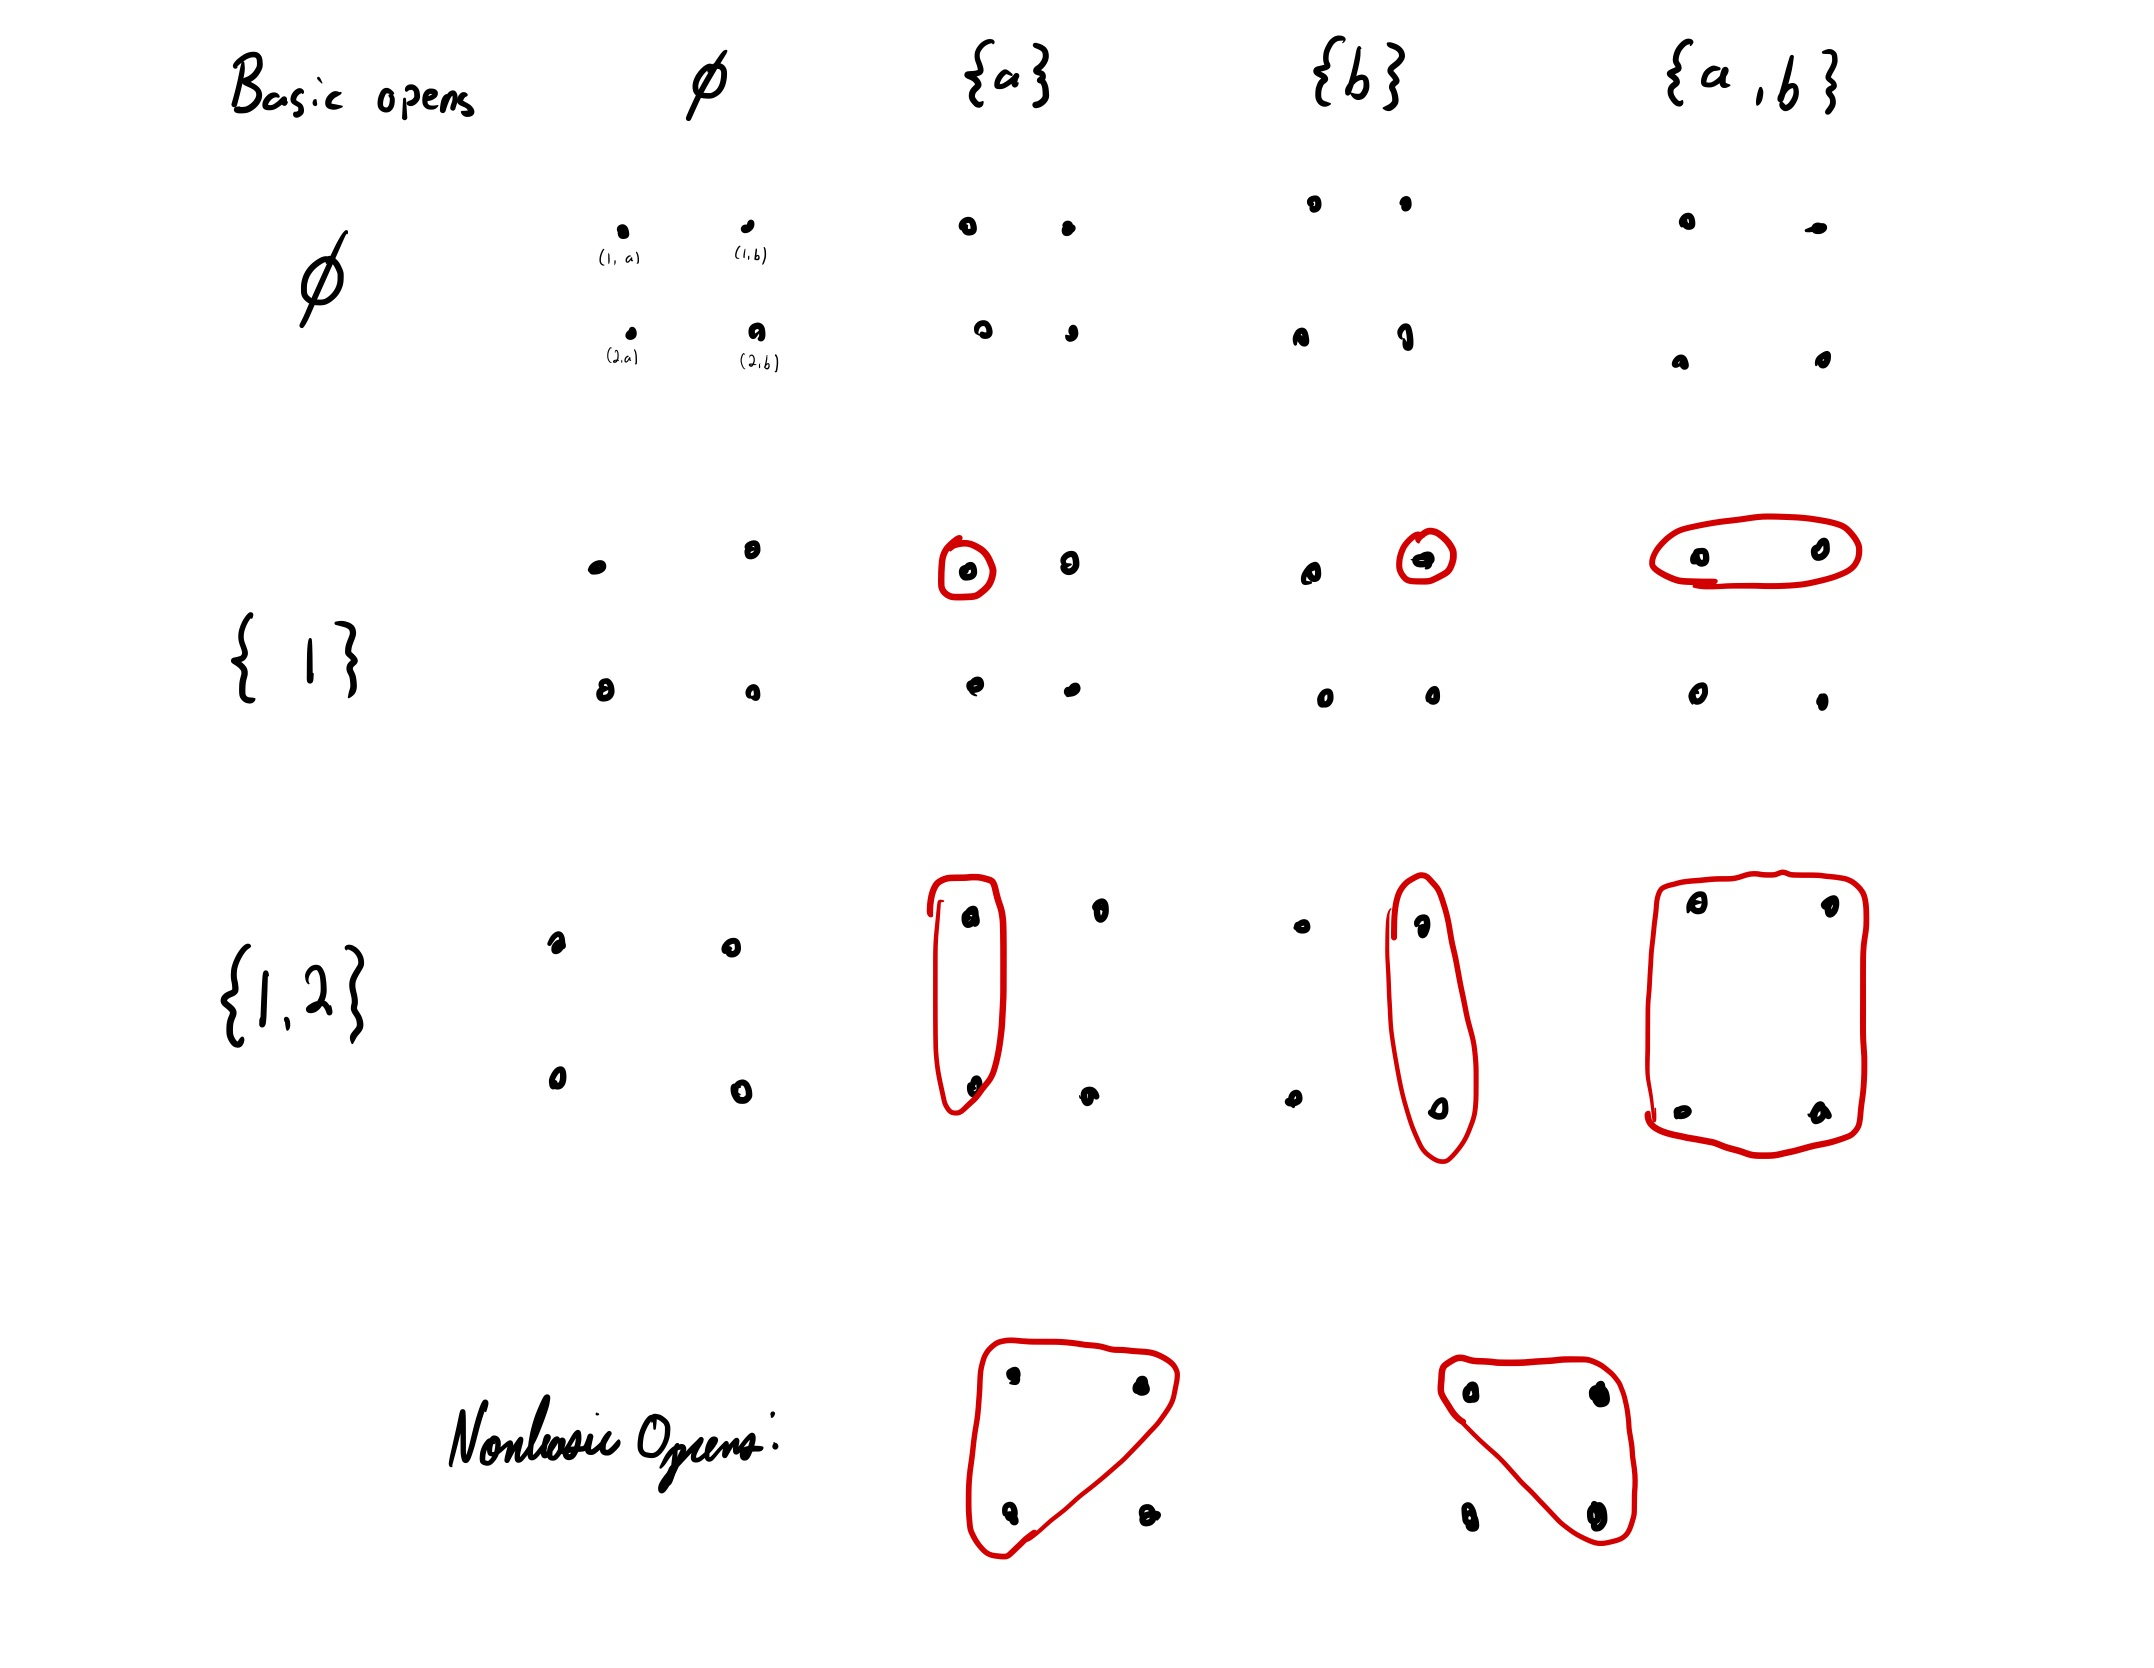
\includegraphics[width=\textwidth]{openchart}
  \caption{All basic and nonbasic open sets}
\end{figure}

Now we continue with the class content, and give a somewhat strange characterization of continuity:

\begin{thm}
  Let \(X, Y\) be topological spaces, \(f: X \to Y\) be a function. Then \(f\) is continuous iff for each subset \(A \subseteq X\), one has \(f(\overline{A}) \subseteq \overline{f(A)}\).
\end{thm}

\begin{proof}
  \begin{enumerate}
  \item [\((\Rightarrow)\)] Suppose that \(f\) is continuous. Let \(A \subseteq X\). Let's show that if \(x \in \overline{A}\), then \(f(x) \in \overline{f(A)}\).

    Let \(V \subseteq Y\) be an neighborhood of \(f(x)\). Let \(U = f\1(V)\). note that \(U \subseteq X\) is open and \(x \in U\), so \(U\) is an open neighborhood of \(x\). Since \(x \in \overline{A}\), there is some point \(x_2 \in U \cap A\). Then \(f(x_2) \in f(U)\)and \(f(x_2) \in f(A)\). Therefore \(f(x_2) \in V \cap f(A)\), so \(V \cap f(A) \neq \emptyset\) and \(f(X) \in \overline{f(A)}\) as desired. \partdone

  \item [(\(\Leftarrow\))] Conversely, suppose that \(f(\overline{A}) \subseteq \overline{f(A)}\) for all subsets \(A\) of \(X\). Let \(B \subseteq Y\) be a closed set. Consider \(A = f\1(B)\). Notice that \(f(f\1(B)) \subseteq B\). If \(x \in \overline{A}\), then
    \begin{align*}
      f(x) \in f(\overline{A}) \subseteq \overline{f(A)} \subseteq \overline{B} = B.
    \end{align*}

    So \(x \in f\1(B) = A\). Then \(\overline{A} \subseteq A\), so \(A = \overline{A}\), so \(A\) is closed, as desired.
    \end{enumerate}
  \end{proof}

  We're going to diverge a little bit now to begin talking about localization, and developing the language around it.

  \begin{lm}
    Let \(f: X \to Y\) be a continuous function. If \(A \subseteq X\) and \(B \subseteq Y\) such that \(f(A) \subseteq B\), then the restriction \(
    \begin{matrix}
      f\vert_A : A \to B \\ a \mapsto f(a)
    \end{matrix}
    \) is also a continuous function.
    \begin{center}
      \begin{tikzcd}
        X \arrow[r, "f"]& Y \\
        A \arrow[u, "i_A"] \arrow[r, "f\vert_A"] \arrow[ur, "f\vert_A"]& B \arrow[u, "i_B"]
      \end{tikzcd}
    \end{center}
  \end{lm}
  This is pretty easy to prove with things that we've done already, so we leave it as an exercise.


  Now it would be nice to express things happening ``near'' a point or ``locally'' on the whole space.

  \begin{exa}
    For example, back in calc 1, given a function \(f: \R \to \R\), \((x, f(x))\) Was said to be a \textbf{local max} if {\color{red}there exists \(\epsilon > 0\)} \(f(x) \geq f(y)\) \sout{for all \(y\) ``near'' \(x\)} {\color{red} for all \(y \in B(x, \epsilon)\)}

    Notice that this is the same as saying:

    \((x, f(x))\) is a local max if there exists an open neighborhood \(U\) of \(x\) such that \(f(x) \geq f(y)\) for all \(y \in U\)
  \end{exa}


  We'll say that something happens ``near'' a point if it happens on an open neighborhood of that point. We'll say that something happens ``locally'' if for all points \(x \in X\) there is an open neighborhood \(U \) of \(x\)  on which something happens.

  In homework, we proved that if \(v \subseteq X\) and \(\opn U_i \cls_{i \in I}\) is a collection of open sets such that \(\bigcup_{i \in I} U_i = X\), then \(V\) is open iff \(V \cap U_i\) is open for all \(i\).

  In other words, a set is open iff it is locally open.

  \begin{df}
    A collection \(\opn U_i\cls_{i \in I}\) of open subsets of a topological space \(X\) such that \(\bigcup_{i \in I} U_i = X\) is called an \textbf{open cover} of \(X\). 
  \end{df}

  \begin{thm}[The local characterization of continuity]
    Let \(f: X \to Y\) be a function between topological spaces, and let \(\opn U_i \cls_{i \in I}\) be an open cover of \(X\)

    Then \(f\) is continuous if and only if \(f\vert_{U_i}: U_i \to Y\) is continuous for all \(i \in I\).
  \end{thm}

  In other words, you are continuous if and only if you are locally continuous.

  \begin{proof}
    \begin{enumerate}
    \item [(\(\Rightarrow\))] Done. \partdone.
    \item [(\(\Leftarrow\))] Suppose \(f\vert_{U_i}: U_i \to Y\) is continuous for all \(i \in I\). Let \(V \subseteq Y\) be an open subset. Then \(f\1(V) \cap U_i = f\vert_{U_i}\1(V)\) for each \(i \in I\). Notice that \(f\vert_{U_i}\) is continuous, \(f\1(V)\) is therefore open.
    \end{enumerate}
  \end{proof}

  One of the reasons we care about localization is because of the study of manifolds, which are spaces which locally look Euclidean. We will talk more about these as the course goes on.

  \begin{thm}
    Let \(X, Y\) be topological spaces. Let \(\opn U_i \cls_{i \in I}\) be an open cover of \(X\).

    \begin{enumerate}
    \item Let \(f: X \to Y\) and \(g: X \to Y\) be functions, then \(f = g\) iff \(f\vert_{U_i} = g\vert_{U_i}\) for each \(i \in I\).
    \item Let \(f_i : U_i \to Y\) be a continuous function for each \(i \in I\), Suppose \(f_i\vert_{U_i \cap U_j} = f_j\vert_{U_i \cap U_j}\) for all \(i\). Then there exists a unique continuous function \(f: X \to Y\) such that \(f\vert_{U_i} = f_i\) for all \(i \in I\).
    \end{enumerate}
  \end{thm}
\end{document}
%%% Local Variables:
%%% mode: latex
%%% TeX-master: t
%%% End:
